\chapter{Software Architecture}
\label{chapter:architecture}

This chapter will discuss the software design behind this work.  It will cover the underlying tools, and then present the framework broken up into functional modules, rather than presenting the entire framework altogether.

\section{Robot Operating System}

The Robot Operating System (ROS)\footnote{\url{www.ros.org}} is a framework for robot software development.  It is a collection of tools and libraries which provides hardware abstraction, device drivers, visualization, message parsing and algorithms relating to robot applications.  ROS is open source software, licensened under BSD.

ROS was selected to be used as the underlying framework for this work to facilitate simpler interfacing with hardware and for recording and playback of video and groundtruth data.  ROS also provides a number of useful tools such as camera calibration.  Finally, using ROS design architecture such as packages and nodes allows better modularity of different software components.  Most of the hardware and libraries utilised in this work already had existing ROS interfaces.

\subsection{ROS concepts}

ROS allows for software to be broken up into separate independant modules, known as ROS \textit{packages}.  These packages may then run as separate executables, also known as ROS \textit{nodes}.  Message types for various datatypes may be defined, which can then be used to allow communication between nodes.  Common interfaces for communication between nodes are ROS \textit{topics} and ROS \textit{services}.

A node may \textit{publish} messages to a given topic.  In this case no feedback is given whether another node has recieved this data successfully or not and therefore no blocking occurs in the node which is publishing.  One or more nodes may \textit{subscribe} to a topic to recieve this information.  Internally, after a node has subscribed to a topic, callbacks will occur when data occurs on this topic.  ROS topics are commonly used for streams of data, such as sensor data.

A service call consists of a request and a response, both of which contain a message which may be defined as per any other ROS message type.  In order to use services, one node needs to become a service server.  The server will listen for service requests from other nodes.  After being called by a service client, the server completes the service and returns the result as the response message.  It must also return a boolean if the service was successful or not.  The service client will wait (blocks) while the server completes the service request.  Services are often used when the client needs a response from another node before it can continue.

Data being published to topics may also be recorded to a ROS \textit{bagfile}.  The bagfile can be replayed and the recorded data will be republished. This is a very useful tool for recording data and playing back sensor data.
 
\section{ScaViSLAM ROS wrapper}

ScaViSLAM is standalone software that does not use any underlying frameworks such as ROS.  Therefore a ROS wrapper for ScaViSLAM was developed. 

\begin{figure}[h]
  \centering
    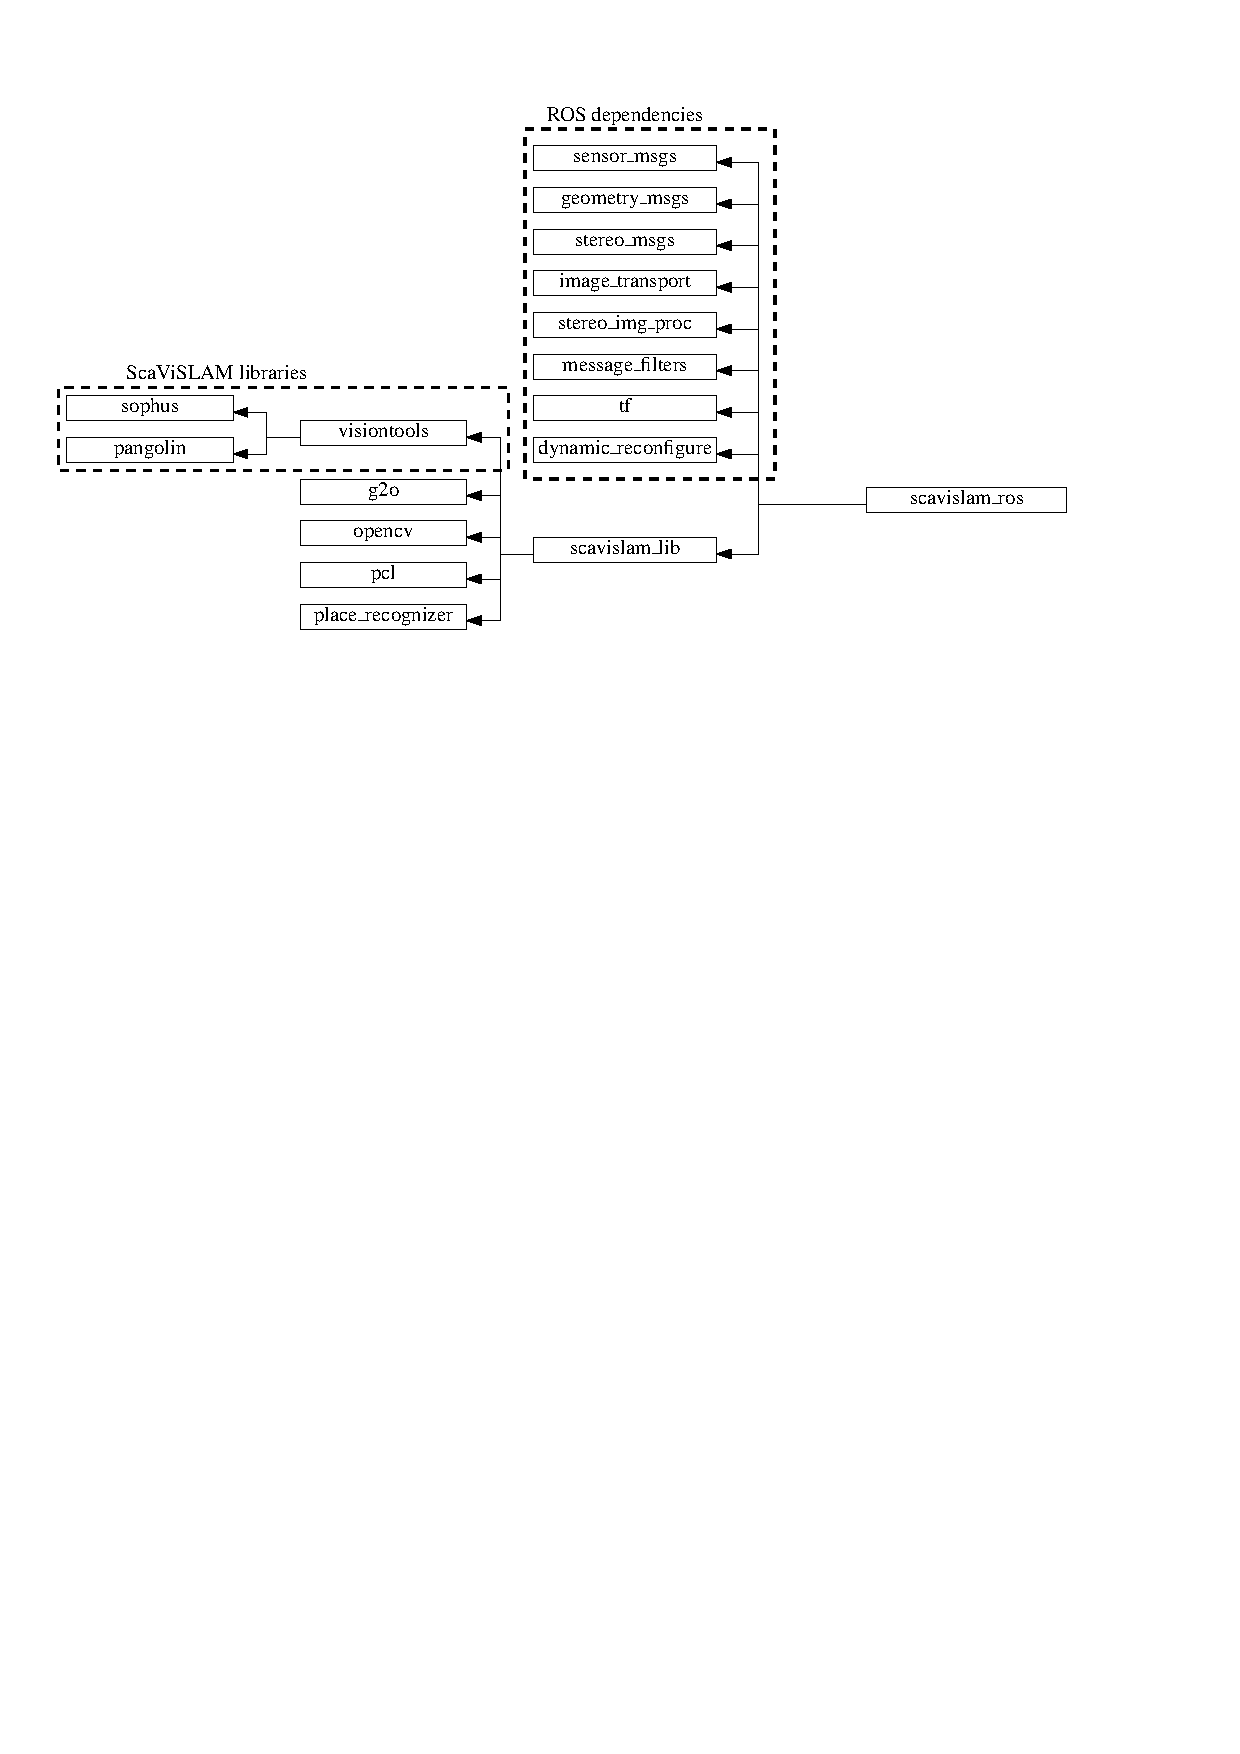
\includegraphics[width=1.0\textwidth]{chapters/images/ros_wrapper_dependencies}
  \caption{ROS package dependencies for the ScaViSLAM wrapper.  scavislam\_lib is designed to have minimal ros dependencies}
  \label{fig:scavislam_wrapper_dependencies}
\end{figure}

In order to do this, ScaViSLAM was split up into two packages; scavislam\_lib and scavislam\_ros.  All of the core functionality of ScaViSLAM was bundled into a library file and contained within the scavislam\_lib package.  To maintain minimal build dependencies and ensure fast compilation and linking, the scavislam\_lib has very minimal ROS code and therefore minimal ROS dependencies.  The scavislam\_ros package contains all of the neccessary ROS dependencies for input, visualization and control using standard ROS tools.  This package acts as a bridge, converting ROS datatypes to ScaViSLAM types and back again. Fig. \ref{fig:scavislam_wrapper_dependencies} shows the ROS package dependencies for scavislam\_ros.  This clearly demonstrates the separation between ScaViSLAM dependencies and ROS dependencies.

This ROS wrapper allows ScaViSLAM to subscribe to standard ROS image topics, which means it can use any stereo camera with a ROS device driver.  It can also use ROS bagfiles containing stereo imagery.  In addition, the ROS wrapper provides a complete replacement of the original ScaViSLAM GUI.  The ScaViSLAM graph may be visualized using rviz, and all visual tracking, keyframes and image pyramids may be visualized either in rviz or image\_view.  All of the original GUI functions may be manipulated using dynamic reconfigure.  More details on the visualization and control can be found under Section \ref{sec:visualization_and_control}

\section{ROS Architecture}

\begin{figure}[h]
  \centering
    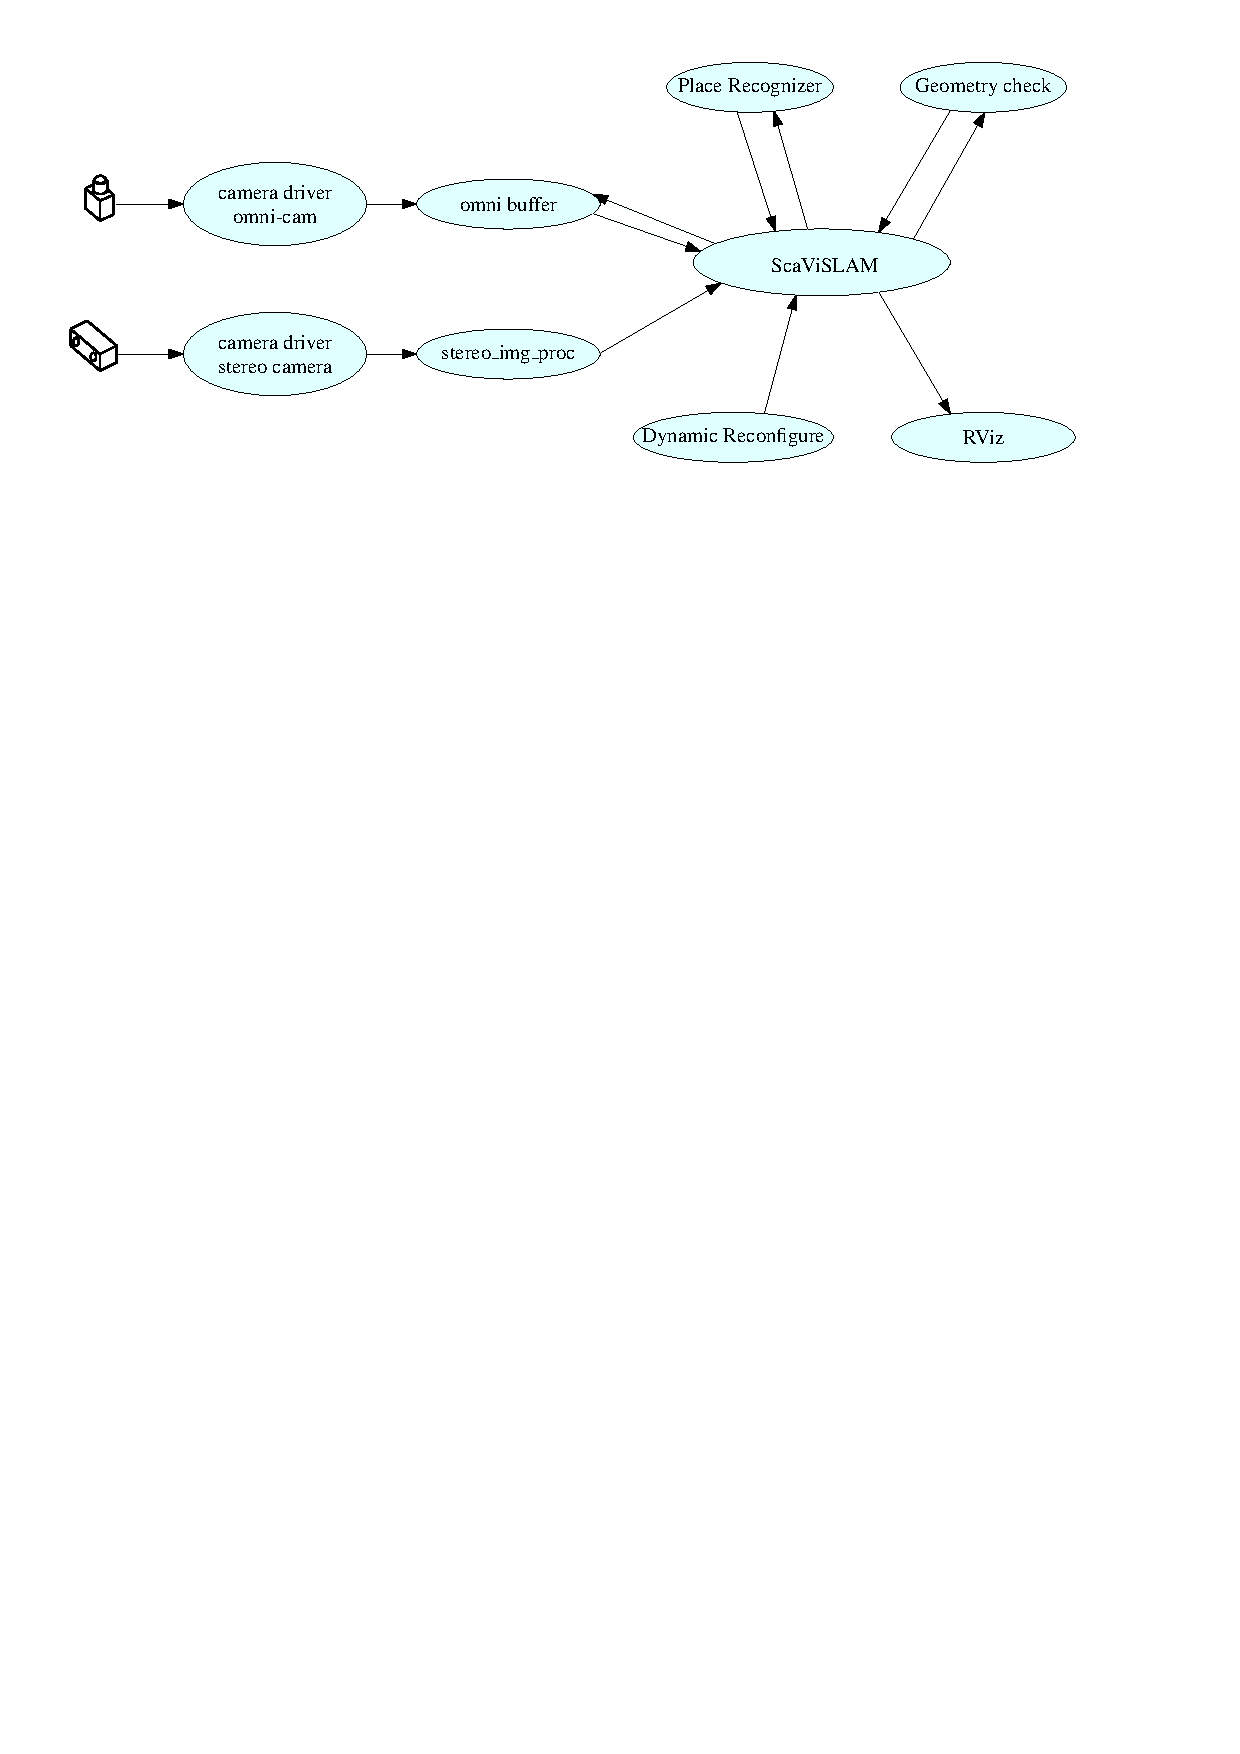
\includegraphics[width=1.0\textwidth]{chapters/images/overall_arch}
  \caption{ROS node diagram for the entire ScaViSLAM system.  Blue ovals are nodes, arrows indicate communication}
  \label{fig:overall_arch}
\end{figure}

Fig. \ref{fig:overall_arch} shows an overall system diagram of ScaViSLAM, showing all the nodes required for the system to run, and the communication between them.  This will be broken down into components in the following sections.

\subsection{Video input}
\label{sec:video_input}

\begin{figure}[h]
  \centering
    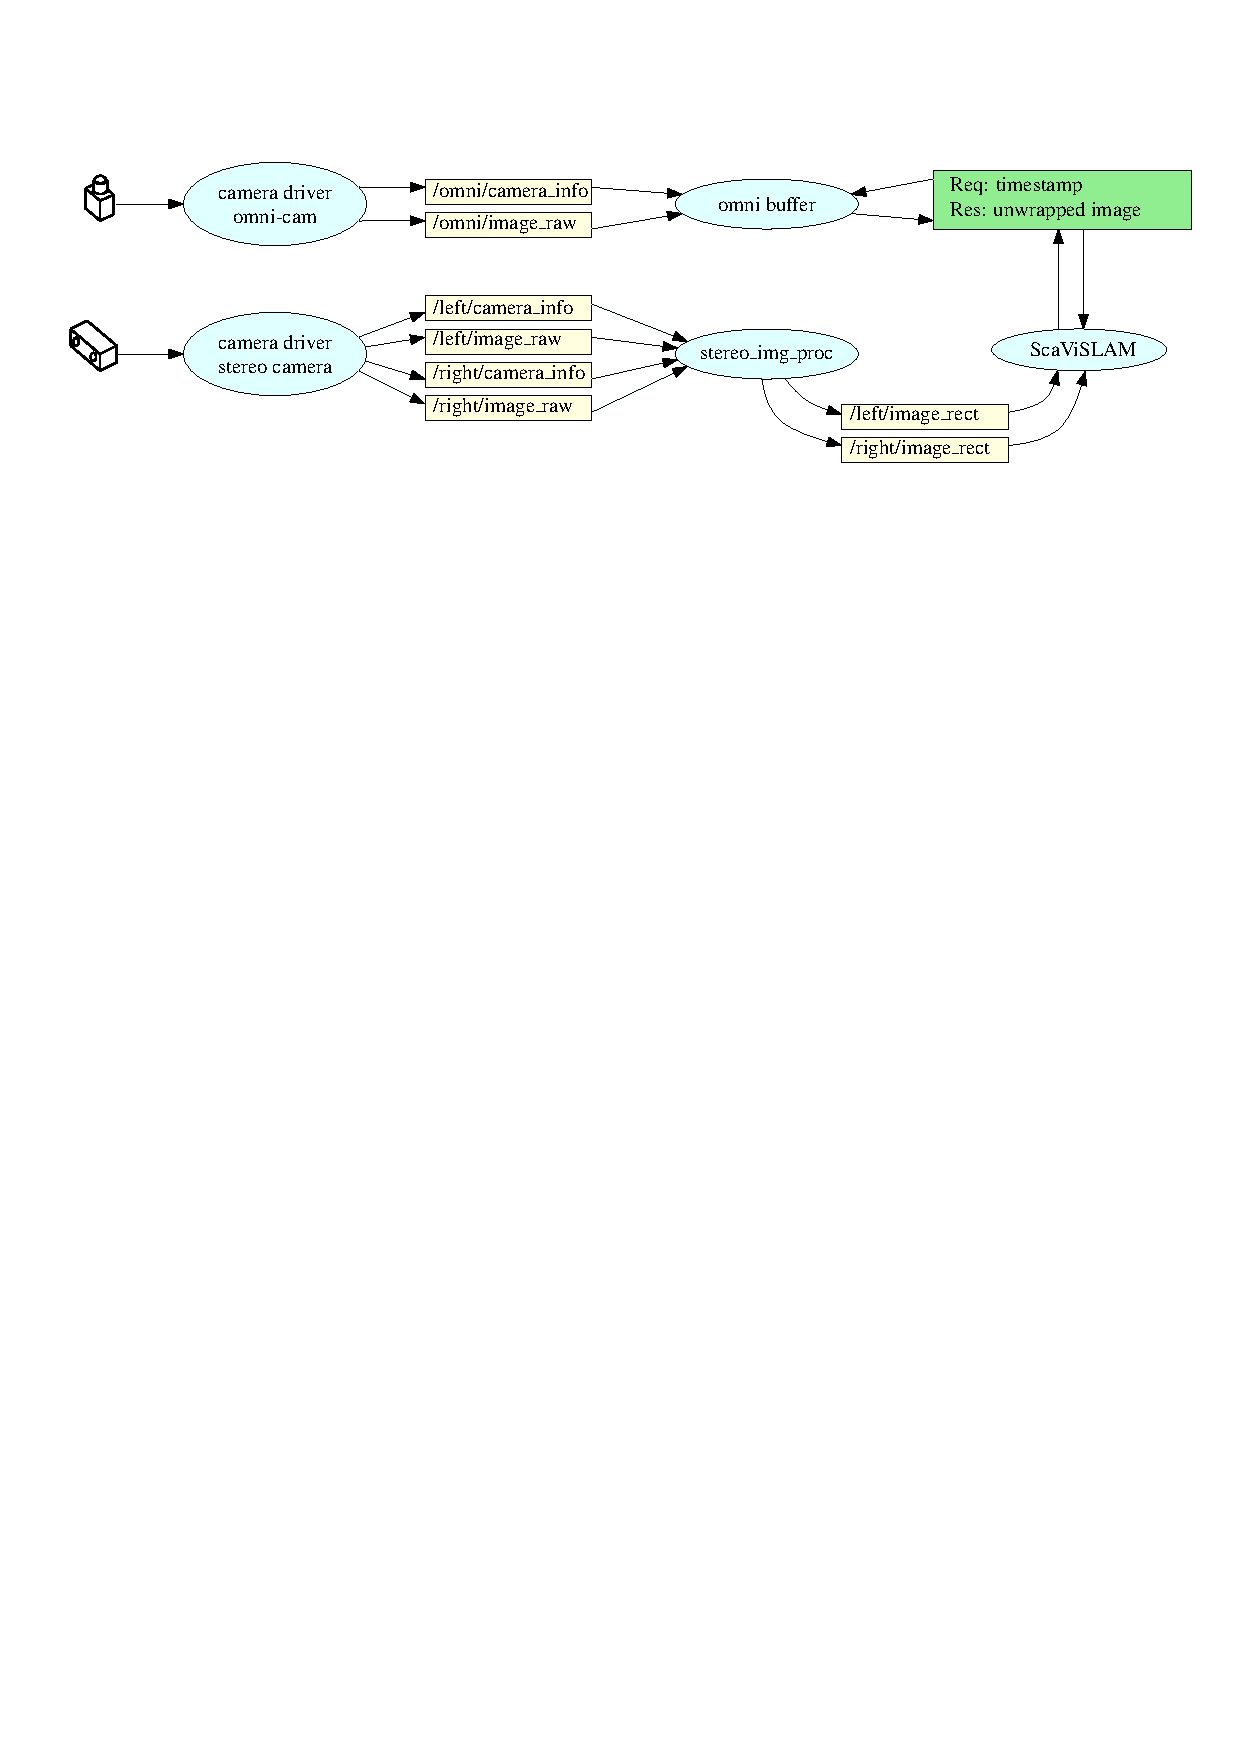
\includegraphics[width=1.0\textwidth]{chapters/images/input_architecture}
  \caption{ROS node diagram for video input to ScaViSLAM system.  Blue ovals are nodes, yellow rectangles are topics and green rectangles are services.}
  \label{fig:input_architecture}
\end{figure}

Fig. \ref{fig:input_architecture} outlines the system architecture for the input to ScaViSLAM.  For the stereo camera, a driver node receives data via Ethernet and publishes raw images and camera info.  The stereo image processing node subscribes to these topics and uses timestamps to ensure the stereo images are appropriately synchronized.  Most importantly, it rectifies the images to non distorted images using the camera intrinsics contained in the camera info message. (For image recitification see Section \ref{subsec:lense_distortion}) 

The pipeline for the omni camera images is significantly different to the stereo frames.  There are two main reasons for this, one being that there was no hardware synchronization available between omni camera and stereo used in this setup, which means that frames could not be accurately synchronized without potentially delaying stereo frames.  The second reason was to increase computational efficiency.  There is some computational load associated with unwrapping donut images to a spherical images.  The omni images are not required for every frame, they are only required for keyframes.  Therefore, only stereo frames which become keyframes require an associated omni camera image.

The omni camera driver receives donut images via firewire and publishes them.  The 'omni buffer' node subscribes to this topic and records every timestamped image to a buffer.  When ScaViSLAM creates a new keyframe, it then queries the omni buffer for an unwrapped image via a service call, providing the timestamp of the stereo frame as part of the request.  The omni buffer node searches through its buffer for the image closest to this timestamp, unwraps it, and returns it as a response to the service call.

This omni buffer node could be configured to unwrap and publish all omni camera frames, however the high resolution omni camera images at 30hz makes processing every frame very computationally expensive.

The ROS tool dynamic reconfigure can be used to configure the camera drivers.  This allows driver parameters to be adjusted, such as gain and shutter controls, resolution and image bit depth.


\subsection{Image based place recognition}

\begin{figure}[h]
  \centering
    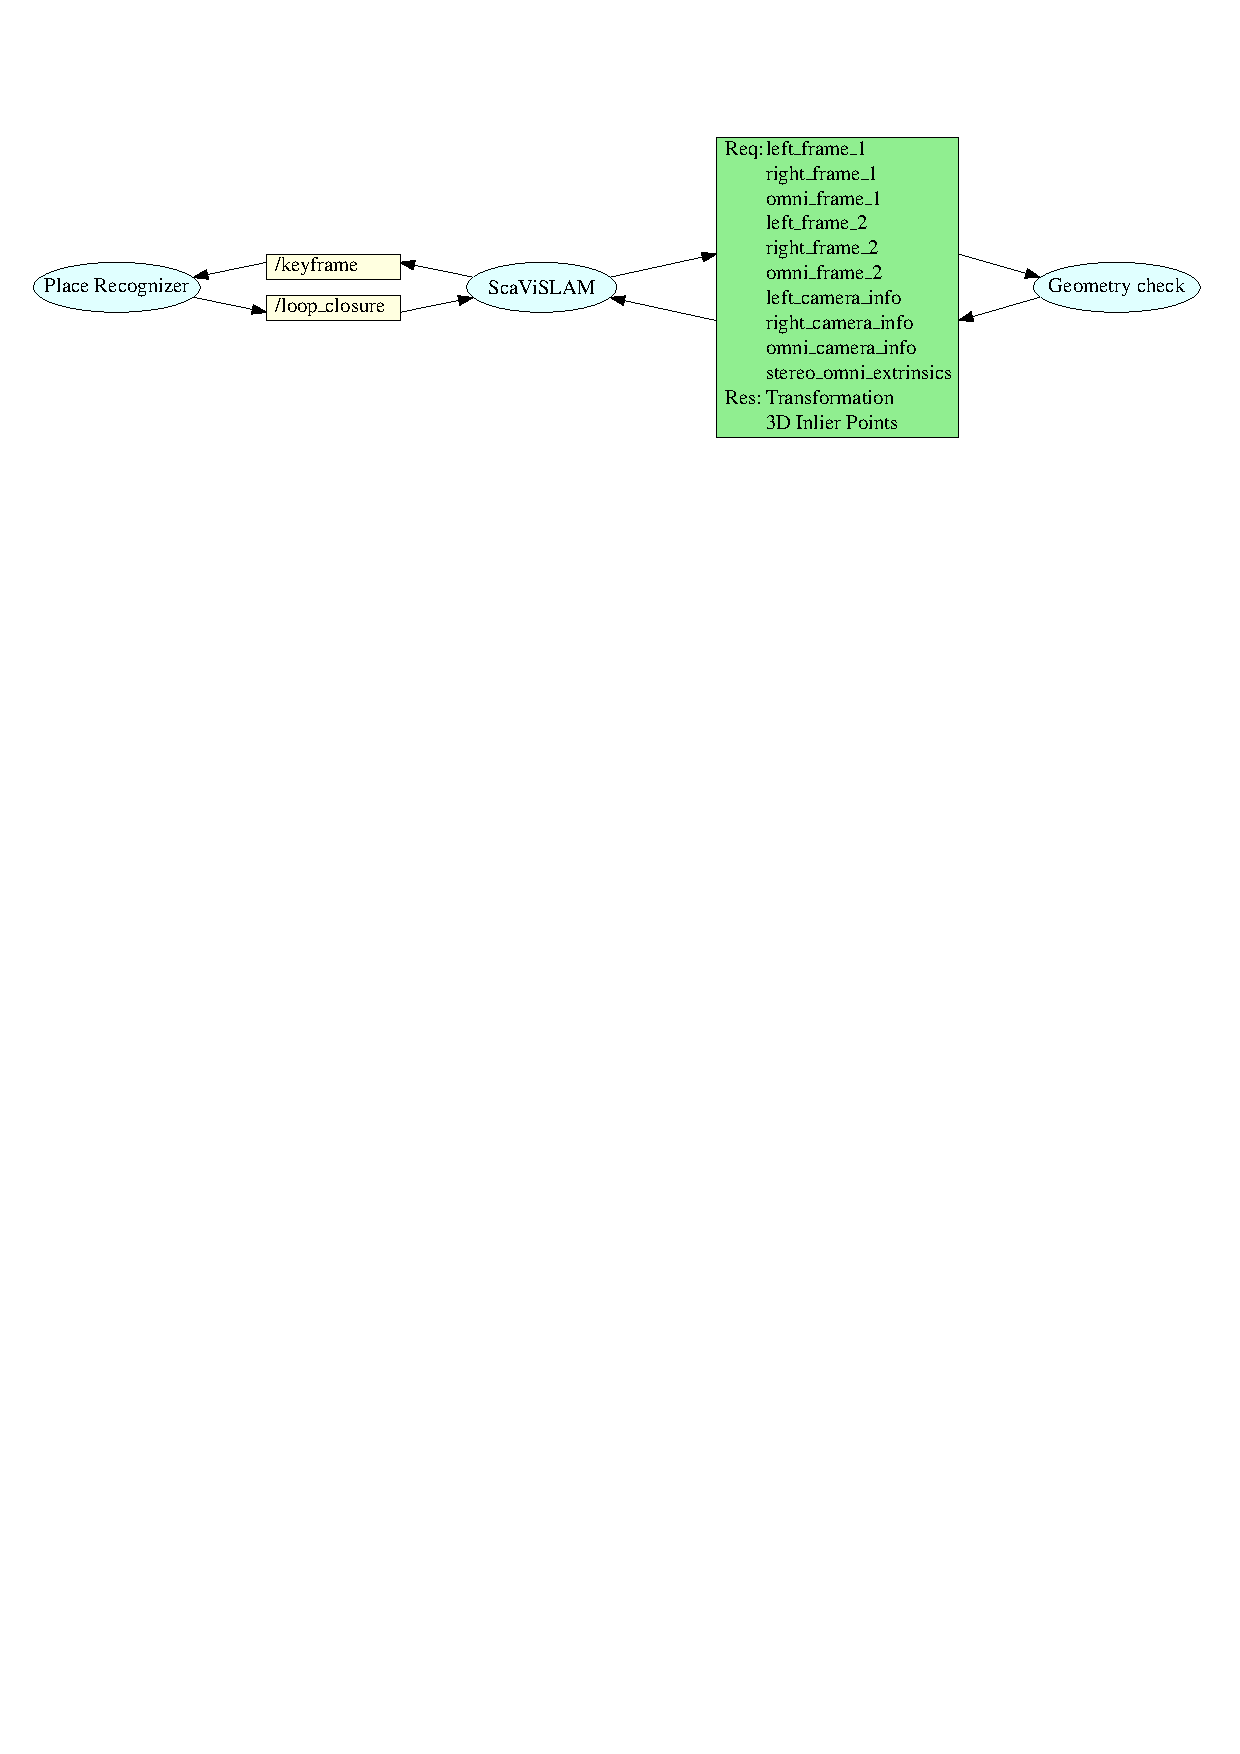
\includegraphics[width=1.0\textwidth]{chapters/images/loop_close_architecture}
  \caption{ROS node diagram for image based loop closure of ScaViSLAM system.  Blue ovals are nodes, yellow rectangles are topics and green rectangles are services.}
  \label{fig:loop_close_architecture}
\end{figure}

The place recognition and geometry check pipeline were both moved into separate nodes from ScaViSLAM, and a successful loop closure involves communication with both.  The motivation for separating the place recognizer node is obvious as it has very clearly defined input and outputs.  Input is a keyframe image and associated ID (/keyframe in Fig \ref{fig:loop_close_architecture}), and output is a pair of ids for a successful match (/loop\_closure in Fig \ref{fig:loop_close_architecture}).  This separation allows easy replacement or modification of the place recognizer implementation without impacting any other code.  It also allows the place recognizer to run in a separate thread.

Although the input output requirements of the geometry check node are not as simple as that of the place recognizer, there are still a number of reasons to also separate it into a different package.  First of all this provides a clear separation between ScaViSLAM code and the omni-loop-closure code developed as part of this work.  Secondly, by taking only images as an input, the geometry check node is agnostic of keyframe ids and keyframe storage specific to ScaViSLAM.  Therefore this geometry check can easily be used by other SLAM systems to perform geometry checks.  The service call shown in Fig \ref{fig:loop_close_architecture} is for an omni-loop-closure.  However the geometry check node also supports stereo pair or mono pair pair geometry checks.  

Finally this architecture allows easy changing between the omni-loop-closure version and the original ScaViSLAM system, which is a requirement for evaluation.  ScaViSLAM only needs to call the stereo pair service instead of the omni-loop-closure service for the original system.

The overall flow for a loop closure is as follows.  ScaViSLAM publishes keyframes as they are created.  The place recognizer encodes a keyframe to the bag of words representation as described in Section \ref{sec:bag_of_words} and associates this new representation with the respective keyframe id.  The original image is then discarded by the place recognizer.  For every new keyframe the place recognizer searches for matching keyframes.  One or more results may then be returned by the place recognizer, in the form of publishing 'potential' loop closure messages, where a single message contains just the two matching ids.  ScaViSLAM subscribes to this potential loop closure topic, and for every ID pair, will obtain all the relevant images from the keyframe storage and then make a geometry check service call.  If the geometry check is successful, then the new edge returned from the geometry check will be added to the SLAM graph.

\subsection{Visualization and Control}
\label{sec:visualization_and_control}

\begin{figure}[h]
  \centering
    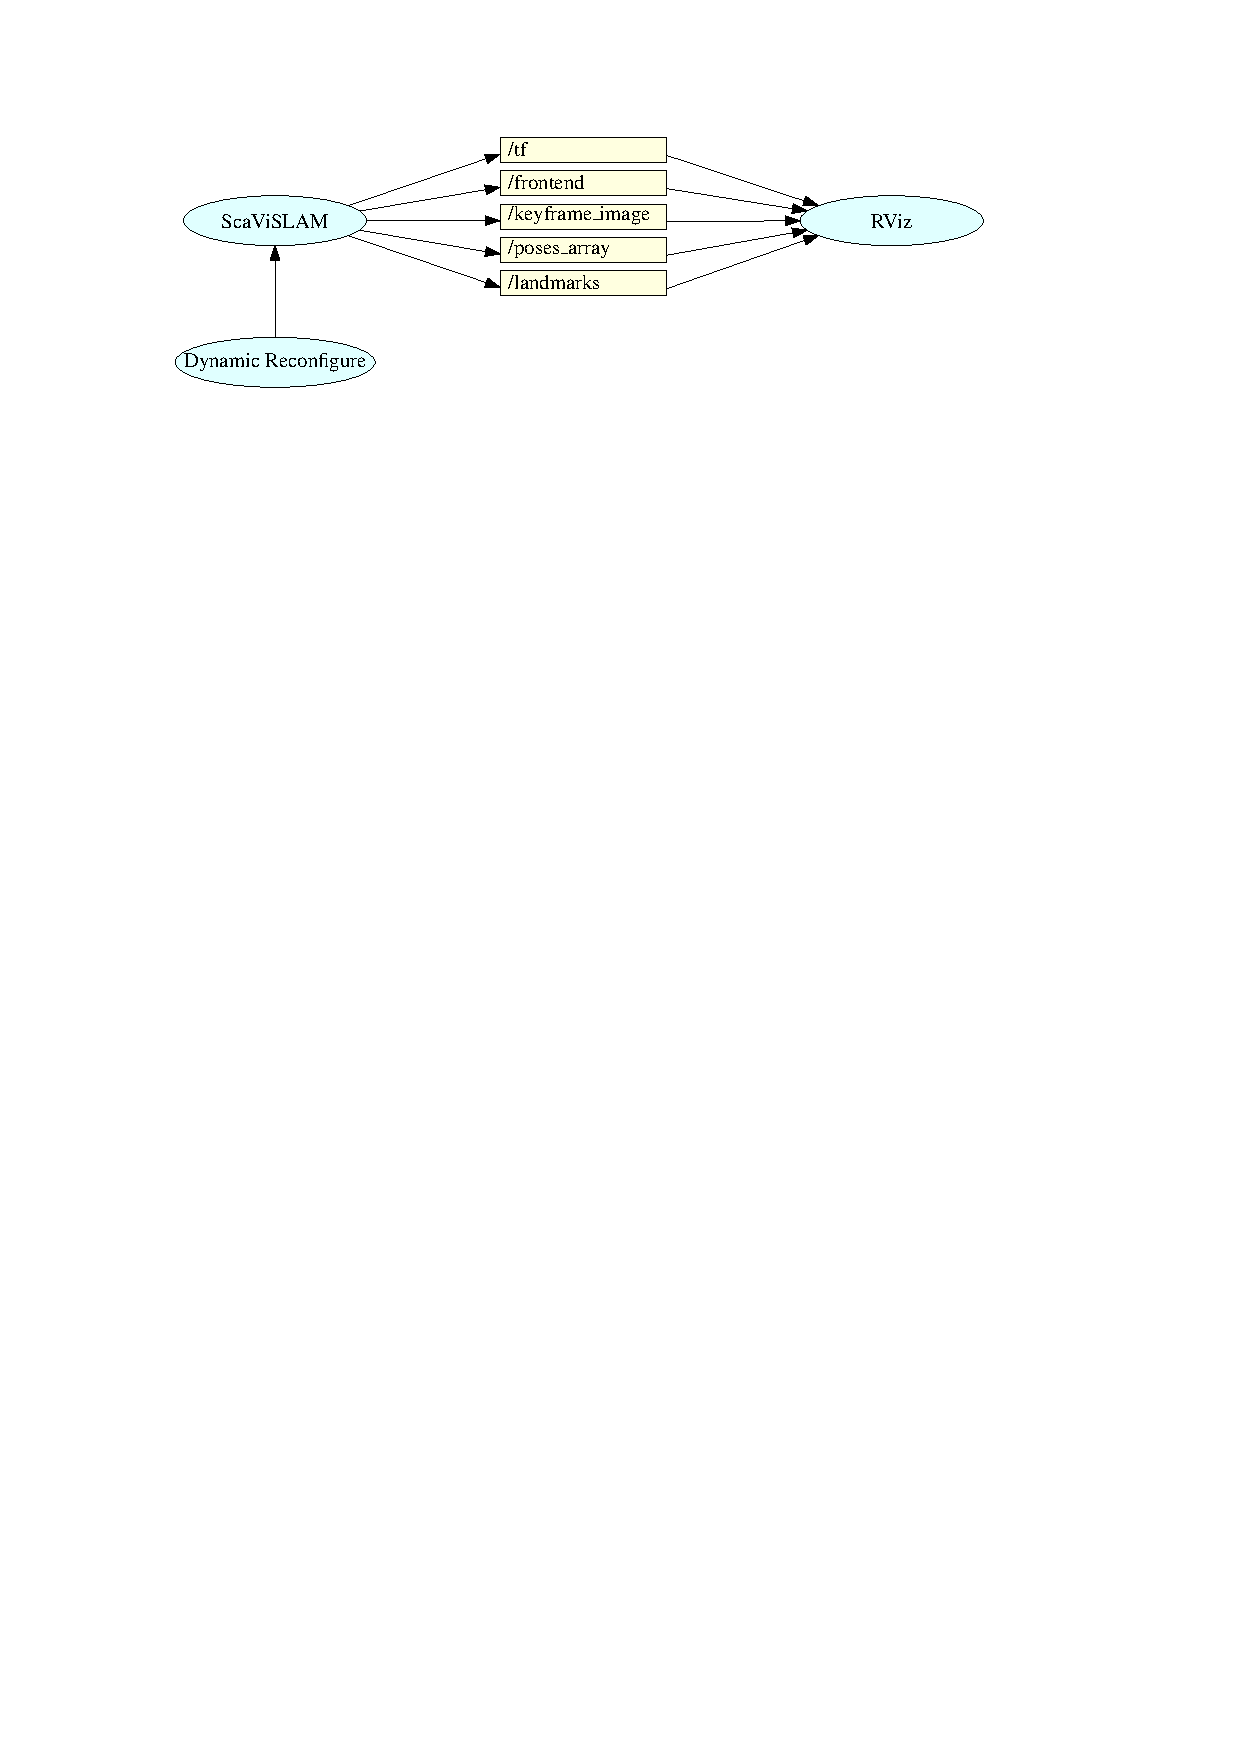
\includegraphics[width=1.0\textwidth]{chapters/images/visualization_architecture}
  \caption{ROS node diagram for visualization and user input.  Blue ovals are nodes, yellow rectangles are topics.} 
  \label{fig:visualization_architecture}
\end{figure}

Fig. \ref{fig:visualization_architecture} depicts the system architecture for visualization and control of ScaViSLAM.  Topics /frontend and /keyframe\_image are image topics.  The /frontend topic shows the visual tracking against the current keyframe and keyframe\_image allows the user to select and show a particular keyframe using dynamic reconfigure.  For both image topics, dynamic reconfigure also allows the user to select which image pyramid level to visualize.

The topics /poses\_array and /landmarks are to visualize the SLAM graph.  The keyframe poses are published to /poses\_array and landmarks within the current inner window are published to /landmarks.  RViz subscribes to these topics and visualizes them.  In addition, the current keyframe and current pose with respect to the current keyframe are published to /tf.  This allows easy comparison with groundtruth data as well as debugging of transformations using RViz.

Control of runtime parameters and visualization options is achieved using dynamic reconfigure.  The actual mechanism of this control is a number of topics and services auto generated by the dynamic reconfigure package and using the dynamic reconfigure GUI tool.  In practice there are too many of these to show here and have therefore been omitted for readability.

%trim = l b r t
\begin{figure}[h]
  \centering
    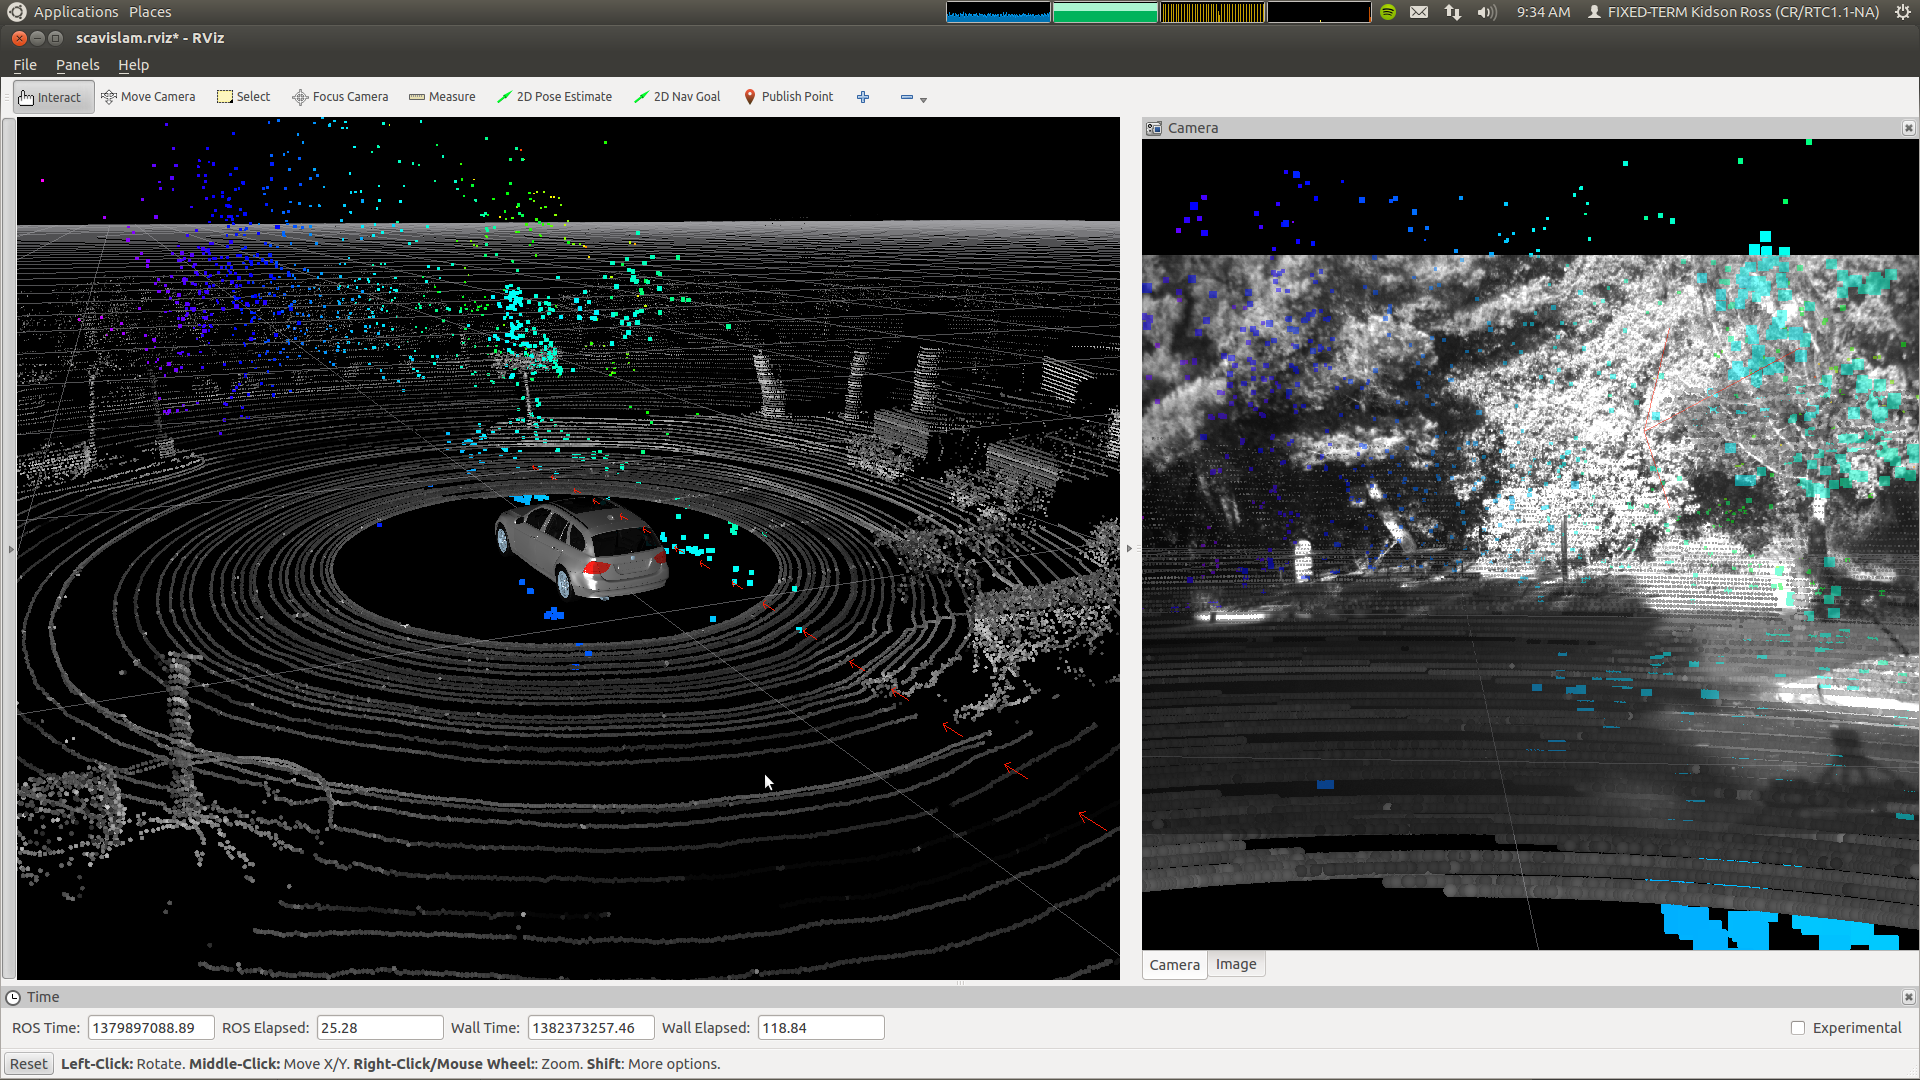
\includegraphics[width=1.0\textwidth, trim=10em 15em 1em 15em, clip=true]{chapters/images/rviz} \\ \vspace{0.5em}
    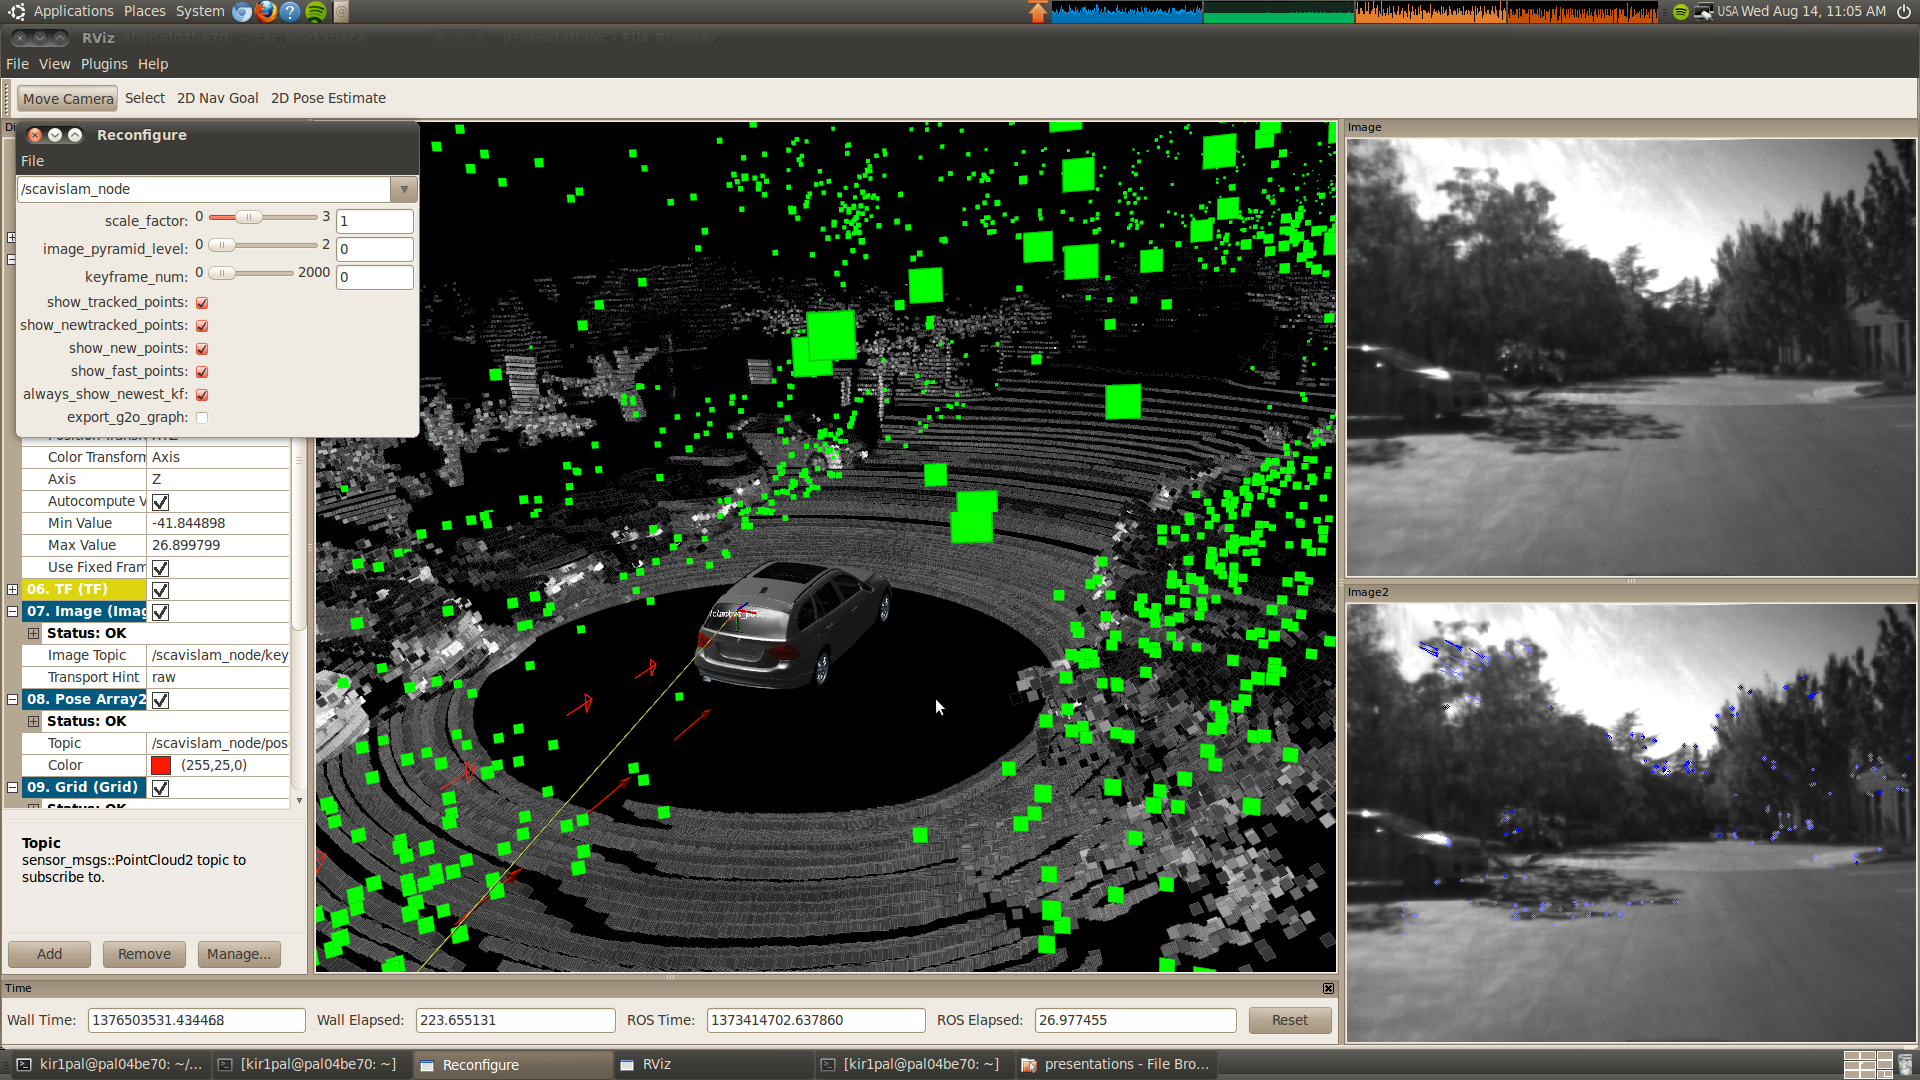
\includegraphics[width=1.0\textwidth, trim=39em 10em 1em 15em, clip=true]{chapters/images/rviz-2}
  \caption{Screenshots of the RViz interface for ScaViSLAM.  Using Rviz to visualize ScaViSLAM allows other sensor data such as point cloud data from a 3D laser scanner to be visualized simultaneously}
  \label{fig:rviz}
\end{figure}